%---------------------------------------------------------------------
%
%                          introduction.tex
%
%---------------------------------------------------------------------
%
% introduction.tex
% Copyright 2015 Dr. Francisco J. Pulido
%
% This presentation belongs to the PhD titled "New Techniques and Algorithms for Multiobjective and Lexicographic Goal-Based Shortest Path Problems", distributed under the Creative Commons Licence Attribution-NonCommercial-NoDerivs 3.0, available in http://creativecommons.org/licenses/by-nc-nd/3.0/. The complete PhD dissertation is freely accessible from http://www.lcc.uma.es/~francis/

\section{Introduction}

\subsection{Motivation}

\begin{frame} 
\frametitle{The Shortest Path Problem (SPP)}
	\begin{block}{Definition}
		The SPP consists in finding a minimal cost path between two nodes in a graph, where the graph is composed of arcs labeled with the cost of the transition between nodes.
	\end{block}
	\begin{itemize}
		\item Solved by Dijkstra in 1959 and by Hart et al. (\astar) in 1968 exploiting specific problem knowledge.
	\end{itemize}
\begin{columns}%[onlytextwidth, t]
\column{0.35\linewidth}
    \begin{block}{Research fields}<2>
    	\begin{itemize}
		\item Artificial Intelligence
		\item Operational Research
		\end{itemize}
    \end{block}
\column{0.45\linewidth}
    \begin{figure}
    \centering
    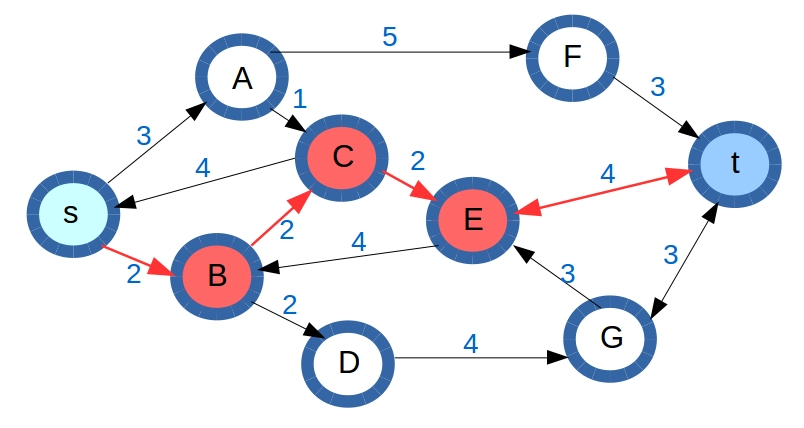
\includegraphics[scale=0.25]{figs/spp}
  \end{figure}
\end{columns}     
\note{The introduction of this thesis begins with the shortest path problem. Given a problem that can be modeled as a graph with nodes representing different states of the problem and the arcs the cost of the transition between those states, the Shortest Path problem is the problem of finding the route with minimal cost between two given nodes, the start and the target nodes.

The Dutch computer scientist Dijkstra in 1959 presented the first algorithm to solve this problem and Hart et al. in 1968 presented \astar, the first optimal algorithm to solve the problem by using specific knowledge acquired from the problem to be solved. Since then, the shortest path problem has been one of the most studied problems in the Artificial Intelligence and Operational Research fields}
\end{frame}
%%%%%%%%%%%%%%%%%%%%%%%%%%%%%%%%%%%%%%%%%%%%%%%%%%%%%%%%%%%%%%%%%%%%%%%%%%%%%%%%%%%%%%%%%%%%%%%%%%%%%%%%%
\begin{frame}[t]  
\frametitle{Applications to the SPP}
  \begin{itemize}
  	\item Path planning in game maps.
  	\vspace{2mm}
  	\begin{itemize}
  		\item The game map is represented as a graph.
  		 \vspace{2mm}
  		\item The characters movement through the map is solved as a SPP.
  	\end{itemize}
  \end{itemize}
  \vspace{4mm}
  \begin{center}
    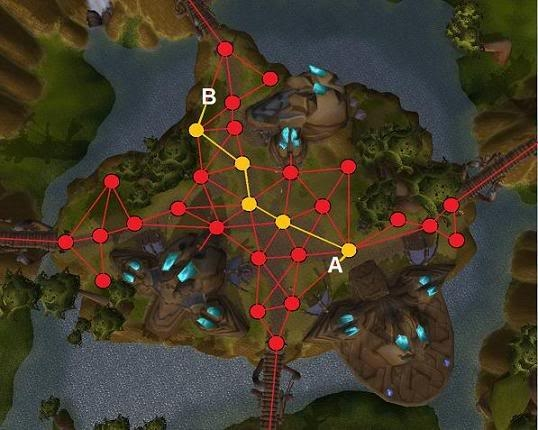
\includegraphics[scale=0.4]{figs/game_maps}
  \end{center}
  \note{One of the typical applications for the SPP is path planning in game maps. As we see in this picture, the possible movements of the characters within the map are represented as a graph.}
\end{frame}
%%%%%%%%%%%%%%%%%%%%%%%%%%%%%%%%%%%%%%%%%%%%%%%%%%%%%%%%%%%%%%%%%%%%%%%%%%%%%%%%%%%%%%%%%%%%%%%%%%%%%%%%%
\begin{frame}[t] 
\frametitle{Applications to the SPP}
  \begin{itemize}
  \item Motion planning in mobile robots.
  \vspace{2mm}
  \begin{itemize}
  		\item The terrain is represented as a graph.
  		\vspace{2mm}
  		\item The robot must find a path avoiding obstacles.
  	\end{itemize}
  \end{itemize}
  \vspace{4mm}  
  \begin{center}
    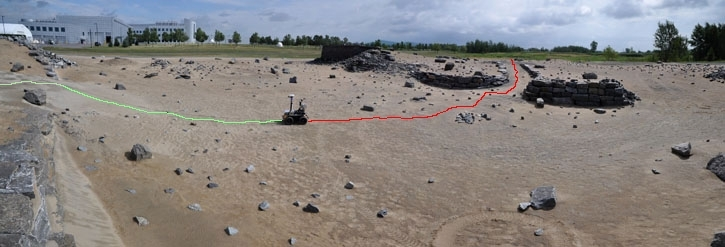
\includegraphics[scale=0.5]{figs/robot}
  \end{center}
  \note{Another application for the SPP is motion planning in mobile robots, where the terrain represents the graph that the robot traverses avoiding the obstacles.}
\end{frame}
%%%%%%%%%%%%%%%%%%%%%%%%%%%%%%%%%%%%%%%%%%%%%%%%%%%%%%%%%%%%%%%%%%%%%%%%%%%%%%%%%%%%%%%%%%%%%%%%%%%%%%%%%
\begin{frame}[t]  
\frametitle{Applications to the SPP}
  \begin{itemize}
  \item Route planning in road maps.
  \vspace{2mm}
  \begin{itemize}
  		\item Real road networks are graphs.
  		\vspace{2mm}
  		\item Arcs represent road junctions.
  		\vspace{2mm}
  		\item Arcs are typically labeled with the distance between junctions.
  	\end{itemize}
  \end{itemize}
  \vspace{3mm}
  \begin{center}
    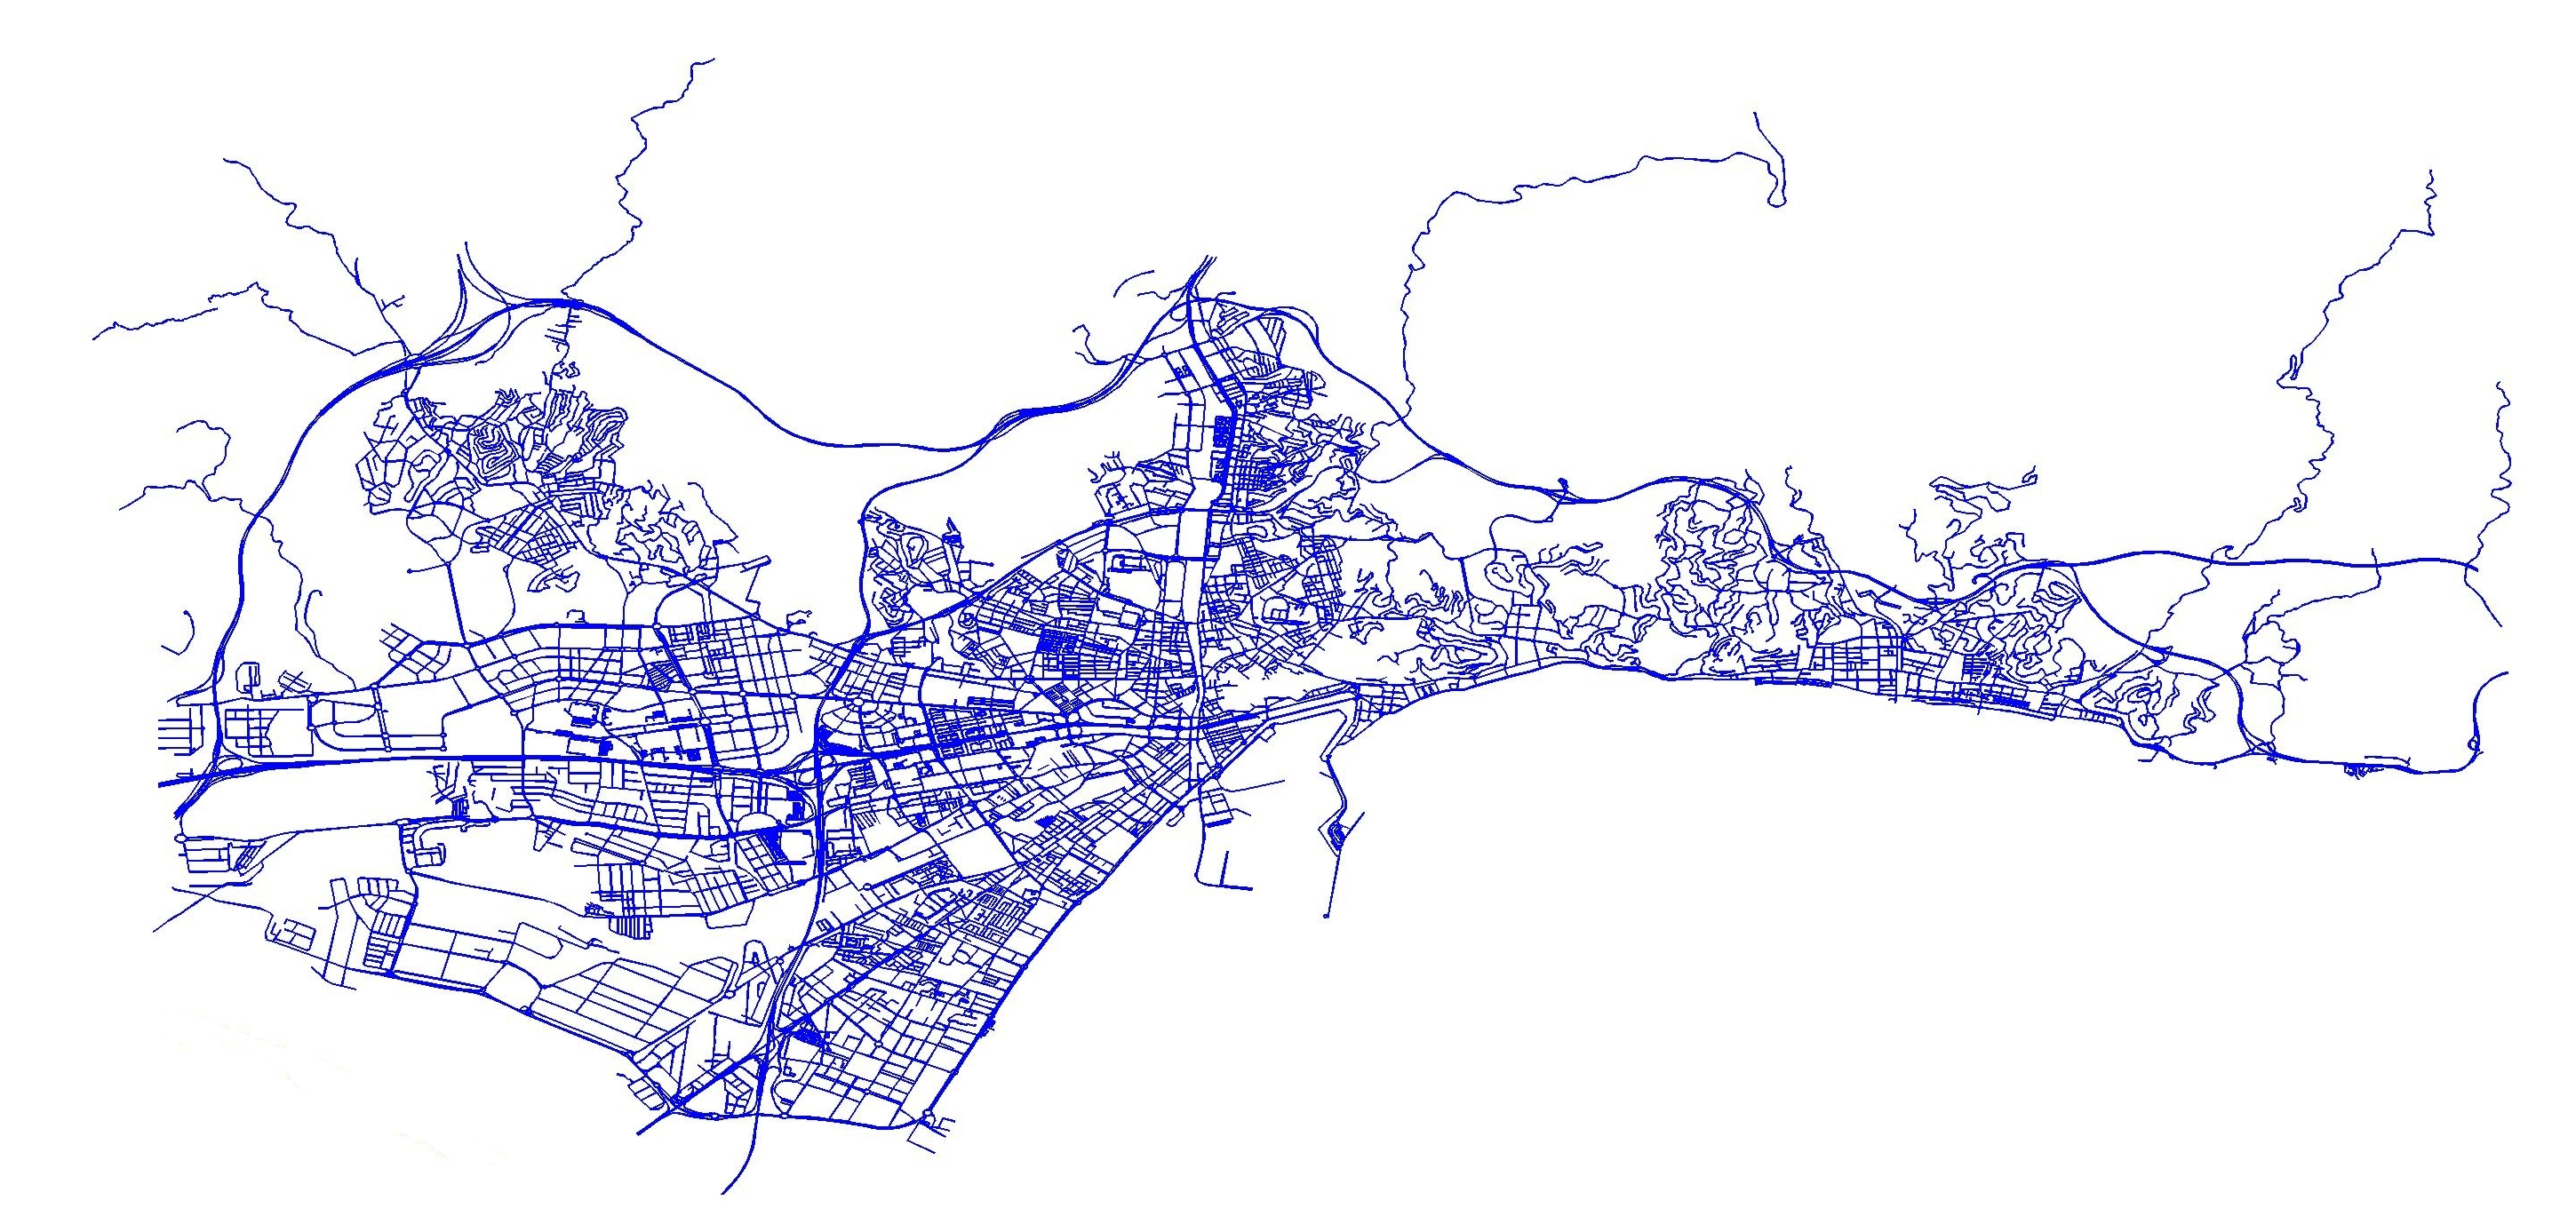
\includegraphics[scale=0.125]{figs/malaga_map}
  \end{center}
  \note{And, perhaps, the route planning in road networks is one of the most natural and studied applications of the shortest path problem. We use in our daily basis google maps or GPS devices to help us plan our trips, and find for us the shortest route to our destination.}
\end{frame}
%%%%%%%%%%%%%%%%%%%%%%%%%%%%%%%%%%%%%%%%%%%%%%%%%%%%%%%%%%%%%%%%%%%%%%%%%%%%%%%%%%%%%%%%%%%%%%%%%%%%%%%%%
\begin{frame} 
\frametitle{Multicriteria Search Problem (MSP)}
	\begin{block}<1->{Definition}
  		\vspace{1mm}
		MSP is the natural extension of SPP to the multicriteria case, where arcs are labeled with \textcolor{ao}{vectors} instead of scalar values.
		\vspace{1mm}	
	\end{block}
	\vspace{8mm}
	\begin{columns}[onlytextwidth, t]
	\column{0.3\linewidth}
	SPP \\
	\vspace{5mm}
	Decision problems 
	\column{0.1\linewidth}
	$\longrightarrow$ \\
	\vspace{5mm}
	$\longrightarrow$ \\	
	\column{0.5\linewidth}
	single-objective optimization problem \\
	\vspace{5mm}
	multiple conflicting criteria
	\end{columns}
\note{SPP has been traditionally considered a single-objective optimization problem. Real decision problems \qquad $\longrightarrow$ \qquad frequently involve multiple conflicting criteria. What is the Multicriteria Search Problem? It's the natural extension of the Shortest Path Problem when several criteria are taken into account simultaneously. The solution to this problem is no longer a single optimal value, but a set of non-dominated or Pareto-optimal paths. We will get deeper into this concept in the following slides, but let's first talk about human decisions.
IMP: Decisions are taken by humans}
\end{frame}
%%%%%%%%%%%%%%%%%%%%%%%%%%%%%%%%%%%%%%%%%%%%%%%%%%%%%%%%%%%%%%%%%%%%%%%%%%%%%%%%%%%%%%%%%%%%%%%%%%%%%%%%%
\begin{frame} 
\frametitle{Human decisions}
	Humans make choices according to their personal preferences, which involve simultaneously multiple, and often, conflicting criteria.
	\vspace{3mm}
	\begin{columns}[onlytextwidth, t]
\column{0.7\linewidth}
	\begin{center}
		
\includegraphics[scale=0.25]{figs/decision}
	\end{center}
\column{0.3\linewidth}
	\only<2->{New car?}
	\begin{itemize}
		\item<2-> Price
		\item<2-> Speed
		\item<2-> Brand
		\item<2-> Color
	\end{itemize}	
	\vspace{3mm}
	\only<3->{A route home?}
	\begin{itemize}
		\item<3-> Distance?
	\end{itemize}
\end{columns} 	

\note{How do we make decisions? We are complex, that's certain, and we make decisions considering multiple criteria, that's certain too. If I'm going to buy a new car, I will consider the price, speed, brand, color... and if I'm checking my GPS device and it is presented to me the shortest route ... it seems that something is missing, isn't it?}
\end{frame}
%%%%%%%%%%%%%%%%%%%%%%%%%%%%%%%%%%%%%%%%%%%%%%%%%%%%%%%%%%%%%%%%%%%%%%%%%%%%%%%%%%%%%%%%%%%%%%%%%%%%%%%%%
\begin{frame} 
\frametitle{Route planning in road maps}
  	\begin{center}
		\includegraphics<1>[scale=0.25]{figs/2}
		\includegraphics<2>[scale=0.25]{figs/3}
		\includegraphics<3>[scale=0.25]{figs/4}
		\includegraphics<4>[scale=0.25]{figs/5}
		\includegraphics<5>[scale=0.25]{figs/6}
		\includegraphics<6>[scale=0.25]{figs/7}
		\includegraphics<7>[scale=0.25]{figs/8}
		\includegraphics<8>[scale=0.25]{figs/9}
	\end{center}
		\note{Let me now present an example of a typical route planning problem. I have finished an important meeting and I will use my fantastic route planning application to find me the shortest path back home.\\
The length of the shortest path from all possible routes is 90 km.\\
Wait! There's a traffic jam on that route and the travel time would be an hour and a half.\\
Maybe, what I do want is not the shortest but the fastest route.\\
This route is 10 kms longer but half an hour faster, it seems to me a good trade-off.\\
or not, there's a toll and this route is 8 euros more expensive than the last.\\
What about a cheaper route?\\
Well, this one is 20 kms longer than the first alternative, 10 minutes slower than the second, but cheaper.}
\end{frame}
%%%%%%%%%%%%%%%%%%%%%%%%%%%%%%%%%%%%%%%%%%%%%%%%%%%%%%%%%%%%%%%%%%%%%%%%%%%%%%%%%%%%%%%%%%%%%%%%%%%%%%%%%
\begin{frame} 
\frametitle{Multicriteria Search Problem (MSP)}
	\begin{block}{Definition}
		\vspace{1mm}
		\textbf{Dominance} or Pareto preference $\prec$: \\
		\begin{center}
		$ \vec{y} \prec \vec{y'} \quad
		\Leftrightarrow \quad
		\forall i \ (1\leq~i\leq~q) \quad y_i \leq y'_i \ \land \ \vec{y} \neq \vec{y'} $ \\
		\vspace{3mm}
		where $ \vec{y} = (y_1, y_2, ..., y_q)$ represents a solution path in the cost space.
		\end{center}
	\end{block}
	\vspace{4mm}
	\begin{example}
		Route cost representation: $\vec{y} = (y_1, y_2, y_3) \ \rightarrow \ \vec{y} = (120, 70, 15)$	
	\end{example}
\note{}
\end{frame}
%%%%%%%%%%%%%%%%%%%%%%%%%%%%%%%%%%%%%%%%%%%%%%%%%%%%%%%%%%%%%%%%%%%%%%%%%%%%%%%%%%%%%%%%%%%%%%%%%%%%%%%%%
\begin{frame}
\frametitle{Pareto optimality}
	\begin{center}
		\includegraphics<1>[scale=0.5]{figs/pareto1}
		\includegraphics<2>[scale=0.5]{figs/pareto2}
	\end{center}
\note{
}
\end{frame}
%%%%%%%%%%%%%%%%%%%%%%%%%%%%%%%%%%%%%%%%%%%%%%%%%%%%%%%%%%%%%%%%%%%%%%%%%%%%%%%%%%%%%%%%%%%%%%%%%%%%%%%%%
\begin{frame} 
\frametitle{Multicriteria Search Problem (MSP)}
	\begin{block}{Definition}
		\vspace{1mm}
		The solution to a MSP, \textcolor{red}{without any knowledge of the user preferences}, is the set of \textcolor{ao}{non-dominated} solution paths, or \textcolor{ao}{Pareto frontier}.
		\vspace{1mm}
	\end{block}
\note{}
\end{frame}
%%%%%%%%%%%%%%%%%%%%%%%%%%%%%%%%%%%%%%%%%%%%%%%%%%%%%%%%%%%%%%%%%%%%%%%%%%%%%%%%%%%%%%%%%%%%%%%%%%%%%%%%%
\begin{frame}
\frametitle{Pareto optimality}
	\begin{center}
		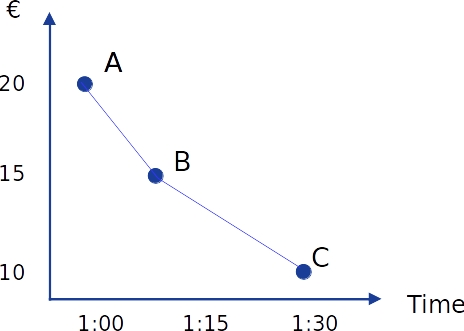
\includegraphics[scale=0.5]{figs/pareto3}
	\end{center}
\note{
}
\end{frame}
%%%%%%%%%%%%%%%%%%%%%%%%%%%%%%%%%%%%%%%%%%%%%%%%%%%%%%%%%%%%%%%%%%%%%%%%%%%%%%%%%%%%%%%%%%%%%%%%%%%%%%%%%
\begin{frame} 
\frametitle{Goal Programming}
	\begin{block}{Definition}
	\vspace{1mm}
		Goal Programming (GP) is one of the \textcolor{ao}{most successful techniques} to solve multicriteria problems. It is also a \textcolor{ao}{natural way to express user preferences} as targets or aspiration levels: $y_i \leq t_i$.
	\vspace{1mm}	
	\end{block}
	\vspace{2mm}
	\begin{block}{Definition}
	\vspace{1mm}
		Lexicographic Goal Programming (LGP) \textcolor{ao}{ranks all goals in order of importance}, dividing them into lexicographic levels of importance.
	\vspace{1mm}
	\end{block}
	\vspace{2mm}
	\begin{block}{Definition}
	\vspace{1mm}
		The deviation from a goal in a minimization problem represents a \textcolor{ao}{positive distance} between the i-th goal and its aspiration level: $d_i = \max(0, y_i - t_i)$.
	\vspace{1mm}
	\end{block}
\note{}
\end{frame}
%%%%%%%%%%%%%%%%%%%%%%%%%%%%%%%%%%%%%%%%%%%%%%%%%%%%%%%%%%%%%%%%%%%%%%%%%%%%%%%%%%%%%%%%%%%%%%%%%%%%%%%%%
\begin{frame}
\frametitle{Goal Programming}
	\begin{example}
		Three criteria (economic cost (euros), travel time (minutes), and distance (km)) grouped in \textcolor{ao}{two priority levels} where level 1 is \textcolor{ao}{infinitely more important} than level 2. The importance of the criteria within a level is defined by \textcolor{ao}{weights} as: 
	\end{example}
	\begin{equation*}
     \begin{array}{cll}
     	\textrm{Level 1:} & cost \leq 15,      & w_1 = 0.5 \\
     					  & time \leq 75 ,     & w_2 = 0.5 \\ 
       	\textrm{Level 2:} & distance \leq 120, & w_3 = 1.
     \end{array}
   \end{equation*}
   \begin{example}
		Let's assume a \textcolor{ao}{solution path} with cost $\vec y = (10, 60, 150)$, \\
		its \textcolor{ao}{deviation} from those goals is $\vec d$ = (0, \textcolor<2>{red}{30)} $\rightarrow$ \\
		$(\max(0, (10 - 15) \times 0.5) + \max(0, (60 - 75) \times 0.5)$, \textcolor<2>{red}{$(150 - 120) \times 1$})
	\end{example}
\note{Let me assume 3 criteria grouped in two priority levels, where the first level is infinitely more important than the second. Goals 2 and 3 share the same importance within level 2. Let's see some examples of vectors and their deviation: the first one (16,16,20) does not have any deviation from goals, none of objectives have overpassed the goals. This vector, however, has deviation of 4 units in the first level. In the last example, we observe deviation in both levels.}
\end{frame}
%%%%%%%%%%%%%%%%%%%%%%%%%%%%%%%%%%%%%%%%%%%%%%%%%%%%%%%%%%%%%%%%%%%%%%%%%%%%%%%%%%%%%%%%%%%%%%%%%%%%%%%%%
\begin{frame}<beamer:0>
\frametitle{Goal Programming}
	\begin{alertblock}{Dominance in GP}
		\vspace{1mm}
		In general, GP models \textcolor{red}{do not guarantee that the solution found is non-dominated}, only that satisfies the goals. However, in this research work we \textcolor{red}{only seek for non-dominated solutions} that satisfy the goals.
		\vspace{1mm}
	\end{alertblock}
\note{}
\end{frame}
%%%%%%%%%%%%%%%%%%%%%%%%%%%%%%%%%%%%%%%%%%%%%%%%%%%%%%%%%%%%%%%%%%%%%%%%%%%%%%%%%%%%%%%%%%%%%%%%%%%%%%%%%
\begin{frame}
\frametitle{Lexicographic goals}
	\begin{center}
		\includegraphics<1>[scale=0.6]{figs/goals1}
		\includegraphics<2>[scale=0.6]{figs/extreme-solutions}
		\includegraphics<3>[scale=0.6]{figs/goals2}
		\includegraphics<4>[scale=0.6]{figs/goals3}
		\includegraphics<5>[scale=0.6]{figs/goals4}
		\includegraphics<6>[scale=0.6]{figs/goals5}
		\includegraphics<7>[scale=0.6]{figs/goals6}
	\end{center}
\note{}
\end{frame}
%%%%%%%%%%%%%%%%%%%%%%%%%%%%%%%%%%%%%%%%%%%%%%%%%%%%%%%%%%%%%%%%%%%%%%%%%%%%%%%%%%%%%%%%%%%%%%%%%%%%%%%%%
\begin{frame}
\frametitle{\lexgo}
	\begin{block}{Definition}
		We define \textbf{lexicographic goal preferences} ($\prec_{G}$) as a partial order relation, 
\begin{center}
$ \vec{y} \prec_{G} \vec{y'} \ \ \Leftrightarrow \ \ \vec{d}(\vec{y})
 \prec_{L} \vec{d}(\vec{y'}) \hspace{2 mm} \lor \hspace{2 mm}
 (\vec{d}(\vec{y}) = \vec{d}(\vec{y'}) \hspace{2 mm} \land \hspace{2
   mm} \textcolor{ao}{\vec{y} \prec \vec{y'}})$
\end{center}
	\end{block}
\note{In order to return the set of efficient solutions we had to define, first, which are those solutions. We define the partial order relation lexicographic goal preferences as: one vector dominates another according to the goals if either its deviation is lexicographically better or their deviations are equal but that the vector dominates the alternative.}
\end{frame}
%%%%%%%%%%%%%%%%%%%%%%%%%%%%%%%%%%%%%%%%%%%%%%%%%%%%%%%%%%%%%%%%%%%%%%%%%%%%%%%%%%%%%%%%%%%%%%%%%%%%%%%%%
\begin{frame} 
\frametitle{MSP with lexicographic goals}
	\begin{block}{Definition}
		\vspace{1mm}
		The solution to a MSP with lexicographic goals is the \textcolor{ao}{set of non-dominated solution paths} that satisfy the goals, or the subset that \textcolor{ao}{minimizes deviation} if these cannot be fully satisfied.
		\vspace{1mm}
	\end{block}
\note{}
\end{frame}
%%%%%%%%%%%%%%%%%%%%%%%%%%%%%%%%%%%%%%%%%%%%%%%%%%%%%%%%%%%%%%%%%%%%%%%%%%%%%%%%%%%%%%%%%%%%%%%%%%%%%%%%%
\subsection{Research goals}
\begin{frame} 
\frametitle{Research goals}
	\large Tackle the MSP with lexicographic goals from two algorithmic perspectives: 
	\vspace{3mm}
	\begin{description}
		\item<2->[A posteriori] Preferences of the decision maker are provided \textcolor{ao}{after} the execution of the algorithm. 
		\vspace{1mm}
		\item<2->[A priori] Preferences of the decision maker are provided \textcolor{ao}{before} the execution of the algorithm.
	\end{description}
	\vspace{4mm}
	\begin{itemize}
		\item<3-> \textbf{A posteriori} algorithms obtain the \textcolor{ao}{whole Pareto frontier} and then, extract the goal-optimal solutions. 
		\vspace{1mm}
		\item<3-> \textbf{A priori} algorithms will return \textcolor{ao}{only goal-optimal} solutions.
	\end{itemize}
\note{This dissertation tackles the MSP with lexicographic goals. Two different approaches are proposed to solve such problem, considering when the goals are taken into account: A priori, where we devise a new specifically design algorithm to return goal-optimal solutions, and a posteriori, performing a full multiobjective search and then extracting the goal-optimal solutions from the Pareto frontier. 
}
\end{frame}
%%%%%%%%%%%%%%%%%%%%%%%%%%%%%%%%%%%%%%%%%%%%%%%%%%%%%%%%%%%%%%%%%%%%%%%%%%%%%%%%%%%%%%%%%%%%%%%%%%%%%%%%%

